\documentclass[]{imag-ms-template}

\title{
{\small Manuscript created with Template for MIT Journals} \\
{Down-regulating the food-Salience Network of chocolate lovers with real time fMRI neurofeedback}
}

\author {Iara de Almeida Ivo,$^{1,2,3\ast}$  Bettina Sorger,$^{1}$ Anne Roefs,$^{2}$ David E.J. Linden$^{3}$\\
{\small $^{1}$Department of Cognitive Neuroscience, Maastricht University,}\\
{\small $^{2}$Department of Clinical Psychological Science, Maastricht University,}\\
{\small $^{3}$FHML, Mental Health and Neuroscience Research Institute, Maastricht University}\\
{\small $^\ast$Correspondence:  i.dealmeidaivo@maastrichtuniversity.nl}
}

\addbibresource{overleaf_neurofeedback.bib}

\begin{document} 

\maketitle 

\keywords{neurofeedback, rt-fMRI, large-scale networks and mindset}

\newpage

\begin{abstract}
  \\ \textbf{Background:} Food cues strongly influence eating behaviour, increasing intake through environmental and social factors. As overeating is a common feature in disordered eating, there is a need for interventions that mitigate the appetite-enhancing effects of food cues. This study tests whether real-time fMRI (rt-fMRI) neurofeedback can down-regulate activity in the core food-salience network – right inferior parietal lobe, left inferior frontal gyrus, left middle frontal gyrus, and left superior frontal gyrus – and reduce food craving. \\ \textbf{Method}Thirty adults with healthy BMI and high chocolate craving were recruited and randomly assigned to true or yoked (sham) neurofeedback. Participants were instructed to down-regulate activity in individually localised top 10\% most responsive voxels of the food-salience network. Success was defined as a reduction in baseline activity in this network.
  \\\textbf{Results:} [To be determined] \\\textbf{Discussion:} [To be determined]
\end{abstract}

\newpage

\section{Introduction}

When it comes to food, our modern environment is one that promotes overconsumption. We are constantly exposed to easily accessible, high-calorie and palatable food signals(\cite{hillObesityOverviewEpidemic2005}). Our environmental context (\cite{jansenCuedOvereating2011b}), the variety of food (\cite{guerrieriInteractionImpulsivityVaried2008, remickInternalExternalModerators2009}), food advertisements (\cite{harrisPrimingEffectsTelevision2009}), and food intake of other people (\cite{hermansMimicryFoodIntake2012}) have all consistently been shown to increase the likelihood of food intake and habitual overeating. In turn, habitual overeating can then lead to excessive weight fluctuations (\cite{jansenCuedOvereating2011b, frankortCravingStopsYou2014}) and promote unhealthy eating behaviours at the population level (such as binge-behaviour  (\cite{jainBulimiaNervosa2025}, \cite{berkmanManagementOutcomesBingeEating2015})). Nevertheless, many individuals exposed to this environment sustain healthy eating behaviours. This observation raises the question of whether there are inherent factors contributing to the development of unhealthy eating behaviours.

Popular theories in eating behaviour propose that the brain’s reward circuitry responds more strongly to palatable, high-calorie foods than to less palatable options, thereby promoting overconsumption (\cite{hillObesityOverviewEpidemic2005}). However, empirical findings are mixed: univariate fMRI studies often fail to detect greater activation for palatable versus unpalatable foods, suggesting that reward value may be represented in distributed patterns rather than absolute activation levels (%. van der Laan et al., 2011). 
Likewise, meta-analyses report inconsistent differences in reward reactivity between individuals with and without obesity (%Pursey et al., 2014; Stice & Yokum, 2016).

Recent work  (\cite{frankortRewardActivitySatiated2012, franssenPowerMindAttentional2020, franssenEffectsMindsetHormonal2022, pimpiniMoreComplexYou2022, kochsItMatterPerspective2023}) has shifted the focus from static reward responsivity to attentional focus as a key driver of neural responses to food cues. Studies by Pimpini et al. (2022) and Kochs et al. (2023) demonstrated that manipulating participants’ mindsets (e.g., health- vs. taste-focus) dynamically modulates brain responses to food cues, with stronger effects than BMI or trait-like characteristics. Our own prior work has identified a food-salience network, comprising parietal and prefrontal regions, that integrates contextual information and allocates attention to motivationally relevant attributes of food cues. Investigating this network and its modulation by cognitive strategies may therefore be more informative than focusing solely on reward circuitry or weight status.

Neurofeedback using real-time fMRI (rt-fMRI) is a promising tool to address network modulation through cognitive strategies as it provides participants with immediate feedback on the activation of targeted brain regions. This enables learning to up- or down-regulate network activity in real time, potentially altering behaviour. Compared to EEG, fMRI types of neurofeedback  precise targeting of distributed networks like the food-salience network, making it particularly suitable for interventions addressing complex behaviours such as food cue responsivity (\cite{pimpiniMoreComplexYou2022, kochsItMatterPerspective2023}).

Several proof-of-concept studies have applied rt-fMRI neurofeedback to eating-related behaviours in sevral populations, such as restrained eaters and individuals with overweight (\cite{schmidtNeurofeedbackReducesOvereating2015, ihssenNeurofeedbackVisualFood2017b, spetterRealtimeFMRINeurofeedback2017, blumeEEGNeurofeedbackTreatment2022}). Recent clinical work using EEG neurofeedback in patients with Anorexia Nervosa (Lackner et al., 2016) and Binge-Eating Disorder (Blume et al., 2022) showed reductions in restrictive behaviour, improvements in emotional competence, and decreases in binge-eating episodes, supporting the potential for neurofeedback as a therapeutic tool.  After downregulation of high beta activity (EEG) during a food cue exposure, authors observed a decrease in the frequency of overeating episodes [Schmidt 2015 and 2016], binge eating episodes and food craving events, as well as improvements in perceived stress among subclinical restrained eaters. These studies demonstrate feasibility but share common limitations: small sample sizes, passive or generalised protocols and insufficient control conditions (often lacking any type of placebo conditions) (\cite{bartholdyPotentialNeurofeedbackTreatment2013b}, Imperatori 2018). 

Building on this groundwork, the present study uses rt-fMRI NF to directly modulate the food-salience network—comprising the right Inferior Parietal Lobe, left Inferior Frontal Gyrus, left Middle Frontal Gyrus, and left Superior Frontal Gyrus — previously identified in a large-scale study with 108 participants (\textbf{insert reference}). We combine this robust group-level network with participant-specific ROIs, tailored to each individual’s functional activation patterns (best voxel selection). During neurofeedback, participants are encouraged to downregulate network activity while viewing personalised chocolate images, with the image’s vertical position lowering proportionally to their neural downregulation as a motivating cue - Motivational Neurofeedback(\cite{ihssenNeurofeedbackVisualFood2017}). To extend previous work and enable stronger causal conclusions of the neurofeedback approach, we include a yoked-feedback control group, where participants were shown a matching participant's brain activity and proportional outcome instead of their own.

Our study investigates if the food-salience network activity can be downregulated to reduce chocolate craving. We test (1) whether neurofeedback-driven downregulation of taste focus reduces the neural activity in the food-Saliency network; and (2) whether neurofeedback affects subjective craving  and actual chocolate intake; and 3) whether the degree of downregulation is related to the level of craving or chocolate intake. This approach provides a mechanistic, neurobiologically grounded method for modifying food signal responsivity, addressing the limitations of previous cognitive and neurofeedback interventions.

% Notes on Neurofeedback studies
% ihssenNeurofeedbackVisualFood2017b 
%                                   - Niklas Ihssen's proof of concept study with David on Neurofeedback of visual food cue reactivity 
%                                   - Findings: 
%                                              neurofeedback is associated with activation decreases in diverse cortical/  subcortical %                                              regions, including key motivational areas. 
%                                              reduction of neural cue reactivity (only bottom-up and not up-down) 
%                                              "Preliminary evidence" reduction of hunger associated with NF
%                                              "Preliminary evidence" association between down-regulation and the degree of hunger 
%                                                                   - Participants reported no difference between subjective feelings %                                                                     of satiety measured before/after each neurofeedback run, t(9) = %                                                                     −0.070, p = 0.473. -  anecdotal evidence in favor of the %                                                                             nullhypothesis that cravings were rated lower after neurofeedback
%                                                                   -   Small sample size/proof of concept
%                                                                   -   Only online evidence - no long term
%                                  - Motivational Neurofeedback (Image size)
%                                  - 10 participants, only females, fasted 4h - only 7 completed whole study
%                                  - Localiser from passive viewing (neutral house images vs food images)
%                                  - Target areas - amygdala, the putamen/caudate, the insula, thalamus and parahippocampal gyrus 
%                                  - No instructions regarding craving
%                                  - Food images were random and not tailored
%                                  - Control: mirror/passive run
%                                  - 
%bartholdyPotentialNeurofeedbackTreatment2013b 
%                                   - Bartholdy's review in The Potential of Neurofeedback in the Treatment of Eating  Disorders: A                                             Review of the Literature  
%                                   - Findings: 
%                                              complete absence of studies testing neurofeedback paradigms in patients with eating                                                      disorders (EDs) 
%                                   - Gap is due to: (in fMRI) -  Complex Cognitions and Networks: While rt-fMRI offers high spatial                                         resolution, complex cognitions involve the coordination of a network of neural regions and not                                         just a single region. Although single region training results in changes in functional                                                  connectivity, it is unclear whether regional connectivity can be modulated directly. Current                                            multivariate techniques used for network-based training are highly specific to individual                                               participants and require extensive preliminary data.
% Imperatori 2018 
%                                   - Imperatory's Review on NF for EDS
%                                   -  Gaps: few studies (13 included); 
%                                   -  no effect on core ED symptoms (body image, BMI); 
%                                   -  no combined modality studies (biofeedback + neurofeedback). 
%                                   - Methodological issues: high risk of bias, lack of blinding, inadequate controls (mostly waitlist; only 1 double-blind NF study), few sessions (mean 7.42; suggest 20-30), no long-term follow-up, high heterogeneity preventing meta-analysis. 
%                                   - Conclusion: preliminary evidence for usefulness in treating dysfunctional eating behaviors (food craving, binge eating) via top-down control and bottom-up salience reduction.
% 

\newpage

\section{Method} 

\subsection{Participants}

Thirty healthy adults (25 women, 5 men) aged between 18 and 48 years (mean = 24.93, SD = 7.37) were recruited through advertisements at Maastricht University. Adults with a BMI between 18.5 and 25, a chocolate-liking score above 75 on a 0–100 scale, and no history of eating disorders were included. After confirming fMRI eligibility (e.g., electronic or ferromagnetic implants, a history of claustrophobia, or panic attacks), participants were invited to a single fMRI session. Participants were instructed to consume a small meal exactly two hours before the experimental session and to refrain from eating or drinking in the two hours leading up to the study. Compliance with this procedure was checked before the scan. All participants had normal or corrected-to-normal vision. The study was approved by the Ethics Review Committee Psychology and Neuroscience of the University of Maastricht, and all participants provided written informed consent prior to participation.

\subsection{Materials \& Measures}

\paragraph{Stimuli:} were selected within an \textit{Image Selection \& Rating Questionnaire}, on Qualtrics. Participants where they were presented with a set of 56 chocolate images. These images were sourced from a local database (database name to be confirmed + add references), featuring a variety of chocolate types, such as dark, milk, and white chocolate, as well as different formats like chocolate bars, truffles, and chocolate-covered snacks. Participants were instructed to select their favourite 25 images and rate each image based on how appealing and desirable they found the chocolate. Rating was assessed using a digital sliding scale ranging from 'Not at all appealing' (0) to 'Very appealing' (100). The chosen top 25 images were used in the main study. This ranking process allowed for the selection of chocolate images that best reflected each participant’s individual tastes, enhancing the ecological validity of the study.

\paragraph*{TCCQ:} The Trait Chocolate Craving Questionnaire (\cite{bentonDevelopmentAttitudesChocolate1998}) was administered as an eligibility criterion during the piloting phase. Eligibility thresholds were defined as scores above 68.6 for women and 48.9 for men, corresponding to one standard deviation above the normative mean (women: 46.8±21.8; men: 29.5±19.4). Using a two-standard-deviation cut-off proved overly restrictive, so it was not applied for inclusion. Nevertheless, TCCQ scores were retained for participant matching.

\paragraph{Craving and hunger ratings:} were completed in person before the scanning session as a brief questionnaire assessing hunger and craving levels. Hunger was rated on a 0–100 Visual Analogue Scale (VAS) with anchors “Not hungry at all” (0) and “Extremely hungry” (100). Craving for milk and dark chocolate was rated separately on a 0–100 VAS (“I do not crave it at all” to “Extremely appealing”).

\paragraph{Bogus Chocolate Taste Test:} Following the neurofeedback session, each participant completed a chocolate taste test designed to measure chocolate consumption. For each participant, their four highest-rated chocolate images from the stimuli selection task were matched to pre-selected commercially available chocolate items. Each item was presented in a standardised portion (e.g., about 50g per piece) on separate small bowls. Chocolates were broken into small portions and weighed before and after the 10-minute tasting period to calculate intake in grams and convert it to kilocalories. Participants were instructed to sample freely and complete a brief questionnaire assessing sensory qualities (taste, texture, sweetness). They were told that the goal of the questionnaire and taste test was to match their image-based preferences to commercial chocolates, in order to create a database of chocolate items with associated questionnaire ratings. While framed as evaluating chocolate products for database development, the primary aim of the task was to measure individual chocolate consumption

\subsection{Participant Matching Procedure}
Participants were allocated to either the neurofeedback or control group using a sequential balancing procedure(\cite{bormSequentialBalancingSimple2005}) to ensure comparability in key demographic and behavioural characteristics. As control participants were presented with yoked feedback derived from the same region of interest selected for their matched neurofeedback participant, allocation proceeded in successive batches (7–7, then 8–8), following a similar procedure to \cite{hamiltonEffectsSaliencenetworknodeNeurofeedback2016}.This design preserved the integrity of the yoked-feedback manipulation, and maintained balanced allocation under the constraint imposed by enrolment order. Details of the allocation procedure and resulting matches are reported in the Appendix (Figure~\ref{fig:participant_allocation_group1}).

\subsection{Session Procedure}
All testing took place in the afternoon, as chocolate is typically consumed later in the day, when craving was expected to be highest. Upon arrival, participants reported on their craving and hunger in a brief written questionnaire. Neurofeedback training was conducted in a single MRI session and consisted of one functional localiser scan and four runs of motivational neurofeedback training. Participants viewed the stimuli via a back-projected screen, visible through a mirror mounted on the MRI head coil. Following the neurofeedback session, each participant completed a chocolate taste test designed to measure chocolate consumption.

\paragraph{Functional localiser:} Participants performed an n-back task with two attentional focus conditions: hedonic and neutral. The localiser block sequence was generated using a constrained randomization procedure, resulting in 12 blocks per condition (24 blocks total) and preventing more than two consecutive blocks of the same type. Each block was introduced by a 1-s block cue, indicating whether participants should focus on tastiness (hedonic) or colour (neutral). Per block, participants were presented with a sequence of six images, each shown for 1.5 s. For each pair of consecutive images, participants indicated via button press whether the current image was more or less colourful (neutral condition) or more or less tasty (hedonic condition) than the previous image. Each response window lasted 1.4s. Responses were not recorded; the primary objective was to maintain active task engagement and attentional focus during the MRI scanning session as suggested by \cite{kochsItMatterPerspective2023}. Within a block there were no repetitions of single pictures. The task was preceded by a 15-s fixation cross, and each block followed the same structure. Based on the statistical contrast between hedonic and neutral conditions in a whole-brain General Linear Model (GLM), we selected for each participant a target area showing reliable activation (top 10\% best voxels across all regions of interest) in the statistical maps derived from the localiser run.

\paragraph{Motivational neurofeedback:} Participants were  presented with chocolate images and were instructed to not focus on taste. Participants were asked to down-regulate activity in the target region while each image was presented. They were informed that the target area was involved in taste processing and were instructed to focus on other attributes of the food images (e.g., colour) rather than taste to achieve regulation. Participants were encouraged to mentally reduce the motivational salience of chocolate and to imagine “swiping” the image downward, and to try different strategies across runs to discover what worked best for them. No specific strategy was enforced, allowing participants to adopt a self-directed approach. This design leverages intrinsic motivation, reinforcing the connection between cognitive control and behavioural outcomes. After each run, participants reported which strategy they used and rated how successful they believed their strategy was for that run on a scale from 0 (“not at all successful”) to 10 (“very successful”).

Neurofeedback was provided intermittently rather than continuously to ensure a clear temporal separation between the regulation period and the feedback period. This approach prevents the movement of the image itself from triggering unintended brain activity, which could bias results. By isolating the participant’s voluntary downregulation efforts, we ensure that observed neural changes are attributable to self-regulation rather than visual motion cues. Instead of conventional feedback methods, such as a thermometer, the stimulus itself served as feedback, making the task more intuitive and engaging.

\subsection{MRI Data Acquisition}

\paragraph{(f)MRI data acquisition} was performed at Scannexus (Ultra-High-Field MRI center, Maastricht, The Netherlands), using a 3T MRI scanner (3T MAGNETOM Prisma Fit, Siemens Medical Systems, Erlangen, Germany) with a 64-channel head coil. Participants lay comfortably in the scanner with their heads stabilised using foam pads on both sides. Stimuli were presented via a mirror attached to the head coil.
A high-resolution T1-weighted anatomical scan was acquired using an optimised magnetisation-prepared rapid gradient-echo (MPRAGE) sequence (TR = 2250 ms, TE = 2.21 ms, flip angle = 9°, FOV = 256 × 192 mm², voxel size = 1 × 1 × 1 mm). T2*-weighted functional images were acquired in an axial interleaved fashion using a gradient-echo echo planar imaging (EPI) sequence (TR = 1000 ms, TE = 31 ms, flip angle = 62°, FOV = 225 mm, voxel size = 2.5 × 2.5 × 2.5 mm, 48 slices). The EPI sequence was optimised to minimise distortion artefacts and susceptibility-related signal loss. The localiser run consisted of 783 brain volumes and each functional run consisted of 532 brain volumes; ensuring whole-brain coverage and high temporal resolution for neurofeedback and cognitive task-based analyses.

\paragraph{Real-time functional imaging} was performed by implementing a custom function in the MR image reconstruction pipeline, which exported pixel data to an additional computer as soon as it became available. TurboExport (version 2.0, Brain Innovation, Maastricht, the Netherlands) was used to transform incoming pixel data for each volume into an image. Each resulting image was preprocessed in real time using Turbo-BrainVoyager (version 4.4; Brain Innovation, Maastricht, the Netherlands). The stimulation computer communicated with Turbo-BrainVoyager via a network connection, using the Transmission Control Protocol (TCP), in order to request the preprocessed real-time data to generate the feedback display. During each neurofeedback block, the percent signal change (PSC) was calculated in real-time for each participant's region of interest (ROI) relative to a baseline referencial period.

The PSC at timepoint $t$, denoted as $\mathrm{PSC}_t$, was computed as:

\begin{equation}
\mathrm{PSC}_t = \frac{PSC_t - PSC_{\mathrm{ref}}}{PSC_{\mathrm{ref}}} \times 100
\end{equation}

where $PSC_t$ is the current BOLD signal intensity in the ROI and $PSC_{\mathrm{ref}}$ is the average signal during the preceding rest period. As such, $\mathrm{PSC}_t$ is expressed in percent units. To translate the PSC into visual feedback, the signal was first normalised relative to a participant-specific baseline value $\mathrm{PSC}_{\mathrm{ref}}$ and an expected signal variation range $\Delta_{\mathrm{PSC}}$. The normalised signal, corresponding to the neurofeedback provided to the participant ($fb$), was computed as:

\begin{equation}
fb = \left( \frac{\mathrm{PSC}_t - \mathrm{PSC}_{\mathrm{ref}} + \Delta_{\mathrm{PSC}}}{2 \Delta_{\mathrm{PSC}}} \right) \times 2 - 1
\end{equation}

This mapping transforms PSC values into the range $[-1, 1]$, with $x_t = 0$ corresponding to the reference level. The reference PSC ($\mathrm{PSC}_{\mathrm{ref}}$) was set per participant as the mean PSC during the hedonic attentional focus condition for the localiser run. This calculation utilised a built-in Turbo-BrainVoyager function that computes percent signal change per condition in real-time. The scaling factor $\Delta_{\mathrm{PSC}}$ was set to 0.5, reflecting an expected maximum deviation of $\pm 0.5$ PSC from reference baseline based on pilot data. %(this range could be adapted per participant based on signal characteristics observed during a calibration phase this week) 

To ensure a stable visual display, the continuous value $fb$ was discretised using 11 evenly spaced steps between $-1$ and $1$:

\begin{equation}
\hat{fb} = \underset{r \in \{-1.0, -0.8, \dots, 1.0\}}{\operatorname{argmin}} \left| x - fb \right|
\end{equation}

The discretised value $\hat{fb}$ was used to determine the vertical position of a visual feedback element (e.g., a food image), which moved smoothly in real time to reflect the participant’s success in modulating ROI activity. Downward movement ($r <0$) indicated successful downregulation of the targeted brain region.



\subsection{Offline Analyses}

\paragraph{MRI data preprocessing} The images were slice scan time-corrected using cubic-spline interpolation, 3D motion-corrected with sinc interpolation and a high-pass filter of three sines was applied. Motion parameters were inspected for quality control. The functional images were co-registered to the anatomical images. Deformation fields derived from segmentation were used to transform all the functional images to Talairach space. Lastly, we performed spatial smoothing with a Gaussian Kernel of 6 mm full width half-maximum (FWHM). Scripts and other tools are publicly available on GitHub at https://github.com/I-ara?tab=repositories.

\paragraph{Neurofeedback Success} was evaluated by quantifying the extent to which participants were able to reduce activation in their individual target brain region. Success was defined in the same manner as online: as a negative deviation in percent signal change (PSC), meaning that activation during regulation phases was lower than during rest phases, relative to each participant’s baseline. For each participant, the degree of success was calculated for every run, and then averaged across the four runs to obtain one mean success score. These mean success scores were then compared between the neurofeedback and the control groups using an independent-samples\textit{ t}-test,  to test whether participants who received real neurofeedback showed greater downregulation than those in the control condition. 

\paragraph{Chocolate Craving} was measured using a single-item rating scale. Participants were asked “How much do you crave chocolate at this moment?” and responded on a 0–100 scale, with higher values indicating stronger craving. A difference score (post–pre) was calculated for each participant to capture craving change across the session. We used a mixed ANOVA with time (pre- vs. post-session) as the within-subject factor and condition (neurofeedback vs. control) as the between-subject factor,  to test whether the reduction in craving was greater in the neurofeedback condition than in the  control condition. Associations between the degree of neural downregulation (downregulation success) and the differential chocolate craving score were examined using Pearson’s correlation.

\paragraph {Chocolate consumption} was measured in kcal to provide an objective index of post-neurofeedback eating behaviour. Neural downregulation success was correlated with chocolate intake using Pearson’s correlation.
\paragraph{Version 1: Independent-samples t-test Chocolate consumption data met the assumptions of normality and homogeneity of variances} Group differences were analysed using an independent-samples t-test. 
\paragraph{Version 2: Mann–Whitney U-test - Chocolate consumption data did not meet the normality assumption or homogeneity of variances assumption}A non-parametric Mann–Whitney U-test was used to compare groups. This test was used to compare mean chocolate intake between groups, as assumptions of normality and equal variances were violated.

\section{Results}

\section{Discussion}

\section{Conclusion}

\section*{Data and Code Availability}

Preprocessing and analysis data scripts can be found at: https://github.com/I-ara?tab=repositories.

\section*{Author Contributions}

Iara de Almeida Ivo: Conceptualization; methodology; formal analysis; software; data curation; writing—original draft; visualisation; project administration.
Anne Roefs: Conceptualization; methodology; formal analysis; writing—original draft; writing—review and editing; supervision; project administration; funding acquisition. 
Bettina Sorger: Conceptualization; methodology; formal analysis; writing—review; supervision; project administration;
David Linden: Conceptualization; methodology; formal analysis; writing—review and editing; supervision; project administration;
Assunta Ciarlo: Sonceptualization; software.

\section*{Funding}

This study is part of the project “New Science of Mental Disorders” (www.nsmd.eu), supported by the Dutch Research Council and the Dutch Ministry of Education, Culture and Science (NWO gravitation grant number 024.004.016). 

\section*{Declaration of Competing Interests}

The authors declare no conflicts of interest.

%\section*{Acknowledgements}
%
%Acknowledgements text (optional).

\section*{Supplementary Material}

Supplementary Material (created during production as a web link to online material).

%Use only to see all references, otherwise print bibliography prints only those used
\nocite{*}
\printbibliography

\appendix

\section{Appendix}

\subsection*{Participant Matching Procedure}
To ensure comparable groups, we matched participants from the control group to the neurofeedback group using a systematic, algorithmic approach. First, we converted categorical variables (sex, chocolate preference) into numerical codes, and scaled continuous variables (age, chocolate liking, chocolate craving) to a 0-1 range using min-max normalisation. This ensured that each factor contributed equally to the similarity calculations.
Next, we computed the Euclidean distance for every possible pair of participants across groups. Each distance represents how similar two participants are across all factors, with smaller values indicating closer similarity. Since the order of factors can influence these distances, we tested all possible permutations of factor order and selected the order that minimised the total distance across all potential pairings.
Finally, to assign participants optimally, we applied the Hungarian algorithm (Munkres, 1957; %via \texttt{scipy.optimize.linear_sum_assignment})
, which finds the one-to-one assignment that minimises the sum of Euclidean distances. This ensured that each participant was paired with the most comparable counterpart, without duplication.
Overall, this approach provided a transparent and reproducible way to create optimally matched participant pairs, with the quality of matches quantified by Euclidean distances in the multidimensional factor space.

\begin{figure}[h!]
\centering
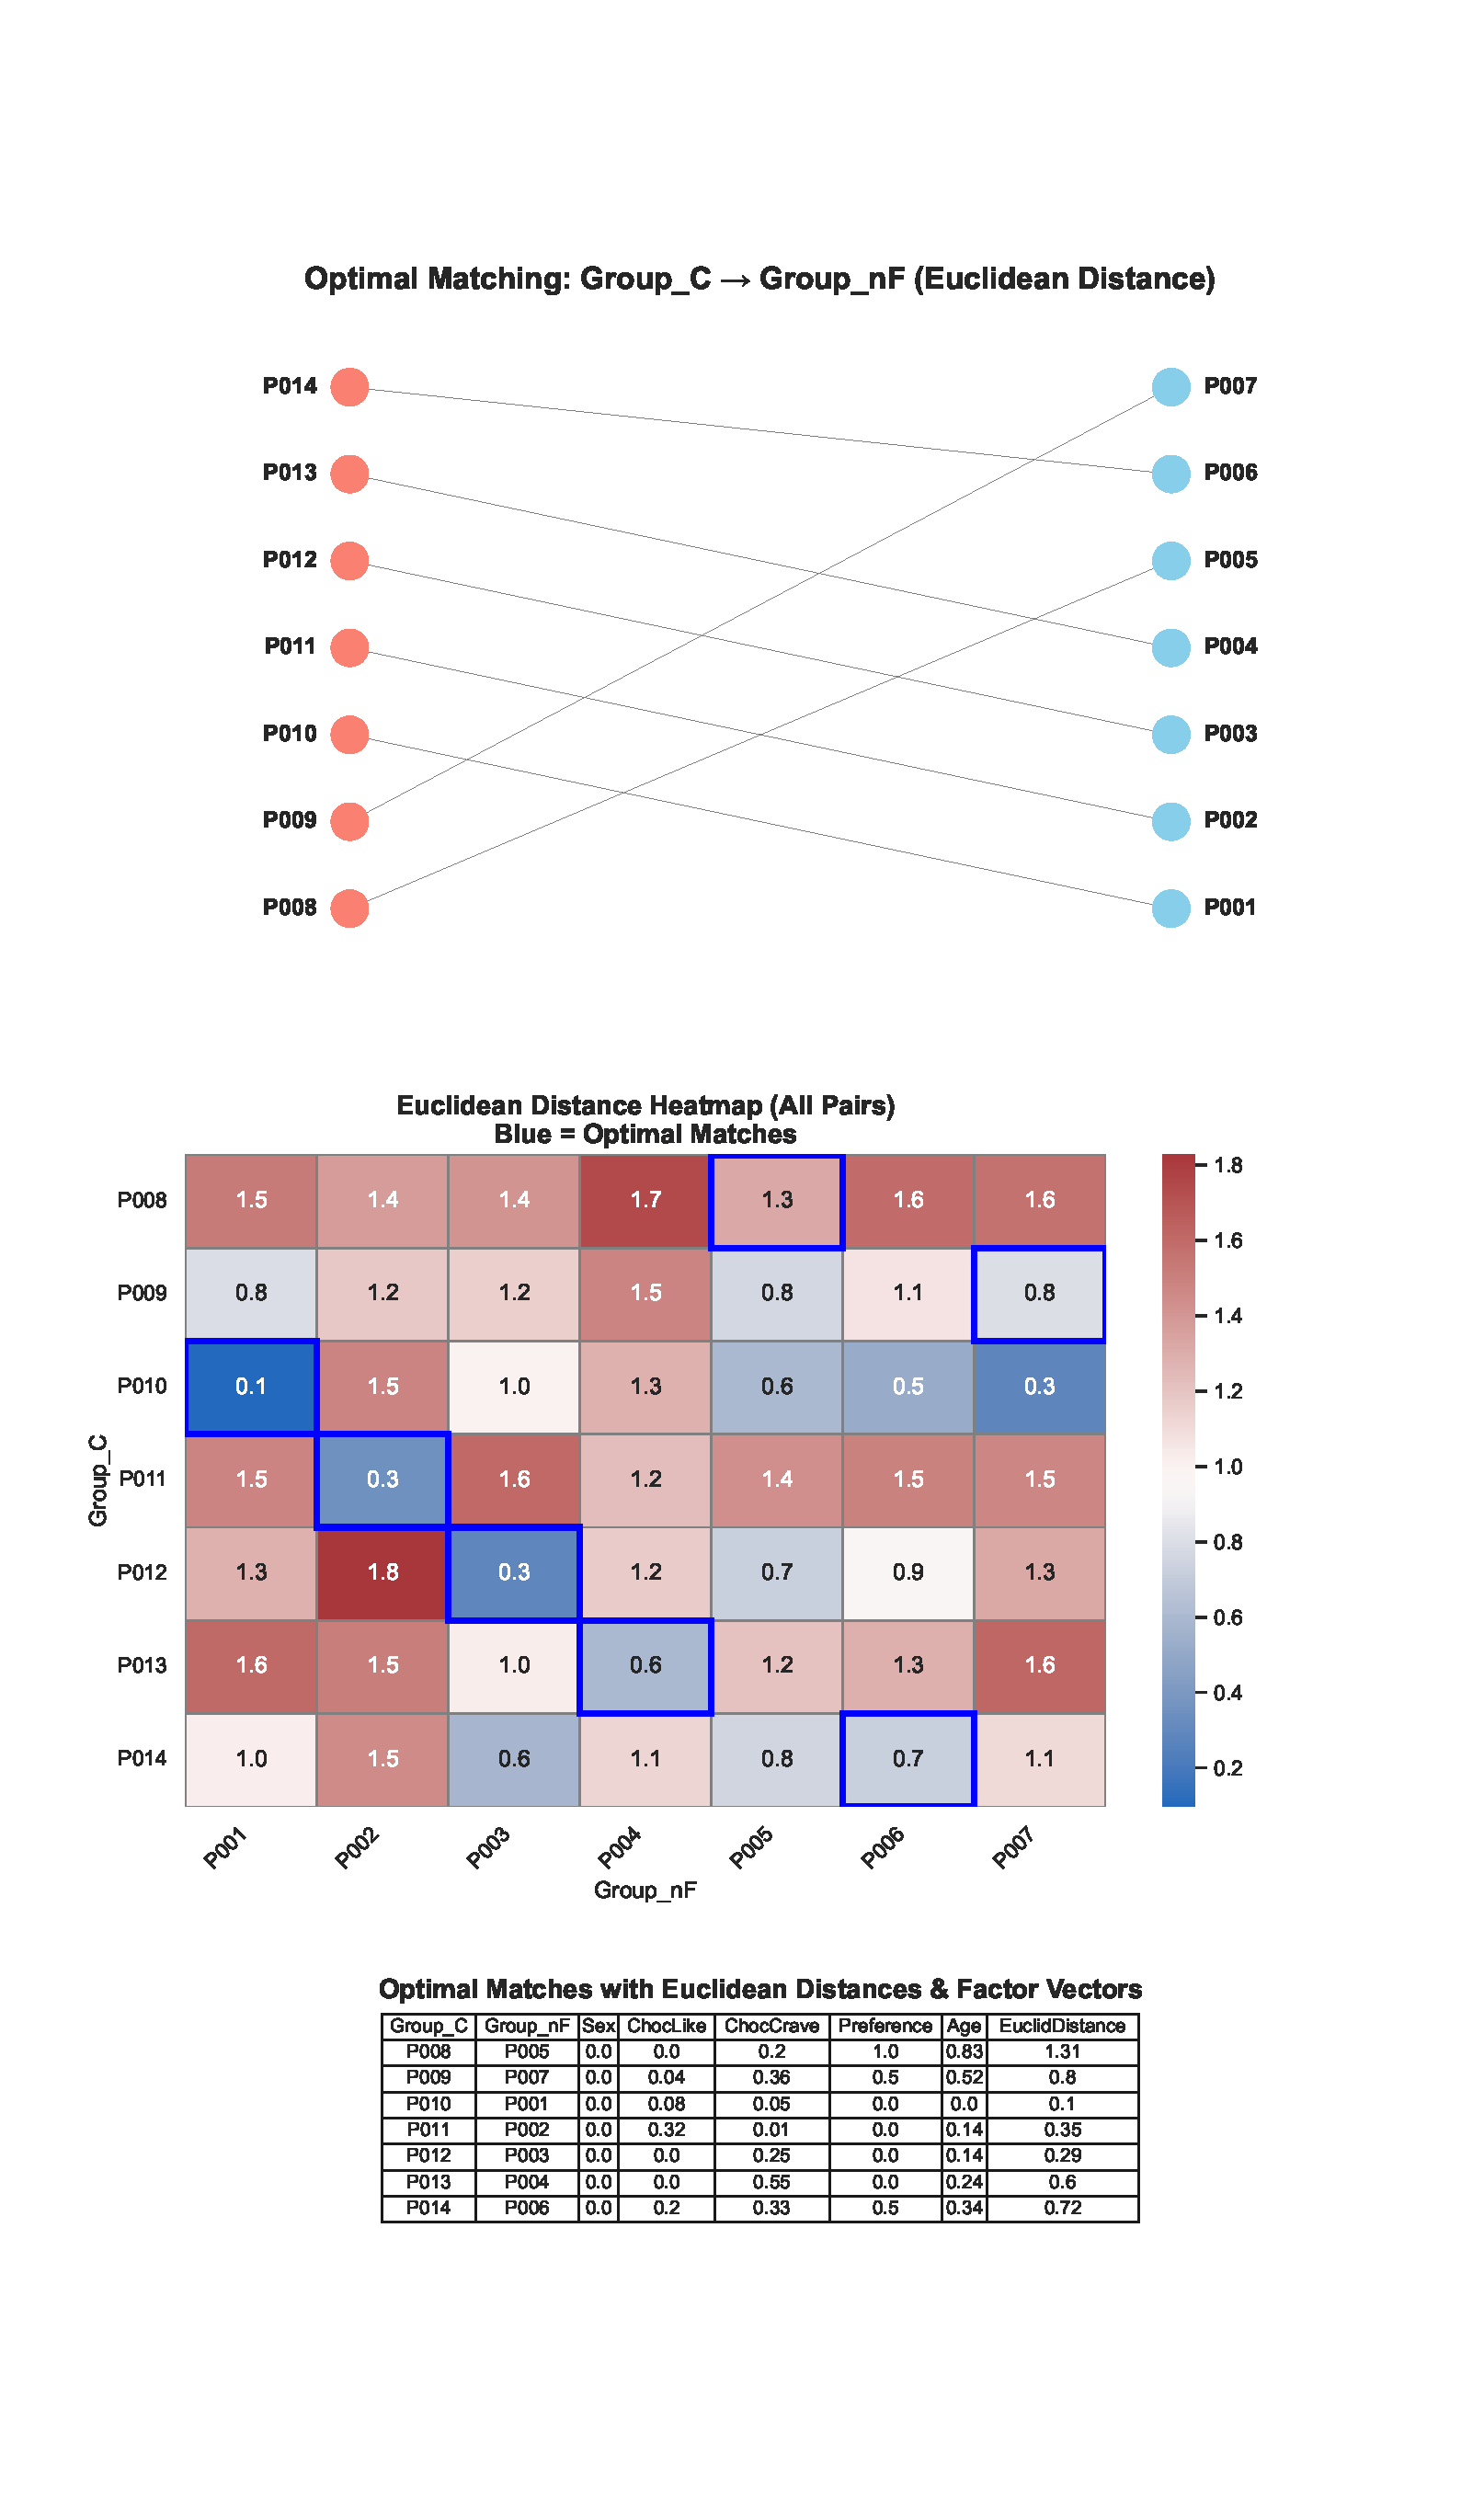
\includegraphics[width=0.8\textwidth,height=0.9\textheight,keepaspectratio]{Matching_14firstparticipants.pdf}
\caption{
Optimal matching outcomes for the first 7 participants in each group (7 vs. 7).  
The figure also shows the Euclidean distances of all matches and the corresponding factor vectors used in the sequential balancing procedure.
}
\label{fig:participant_allocation_group1}
\end{figure}


\textbf{References}
\begin{itemize}
    \item Munkres, J. (1957). Algorithms for the Assignment and Transportation Problems. \textit{Journal of the Society for Industrial and Applied Mathematics}, 5(1), 32--38.
    \item Pedregosa, F., Varoquaux, G., Gramfort, A., et al. (2011). Scikit-learn: Machine Learning in Python. \textit{Journal of Machine Learning Research}, 12, 2825--2830.
    \item Virtanen, P., Gommers, R., Oliphant, T. E., et al. (2020). SciPy 1.0: Fundamental Algorithms for Scientific Computing in Python. \textit{Nature Methods}, 17, 261--272.
\end{itemize}



\end{document}
